\documentclass[runningheads]{llncs}

\usepackage[dvipdfmx]{color}

\usepackage[dvipdfmx]{graphicx}
\usepackage{tikz}

\begin{document}

\section{In the case of $\delta \geq 2$}

\subsection{In the case of $\delta = 2$}

We discuss when the length of seed is $n$. If the length of seed is $n$, the seed will be in an equilateral hexagon with a radius of $n$ when it is given. We will begin our disscussion by considering the moment when a first bead is fixed on a side of an equilateral hexagon with a radius of $n+1$. There are two ways to in Fig.1. fix a bead on a side of an equilateral hexagon with a radius of $n+1$.\\
A dotted line: A hydrogen bond.\\
A dashed line: A side of an equilateral hexagon.\\
A cross: A bead already making a hydrogen bond and cannot make any more

\begin{figure}
  \begin{center}
    \begin{tabular}{cc}
      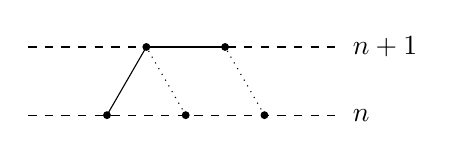
\begin{tikzpicture}
        \draw [dashed] (-1.0, 0.0) -- (3.0, 0.0);
        \fill (3.0, 0.0) node [right] {$n$};
        \draw [dashed] (-1.0, 0.866) -- (3.0, 0.866);
        \fill (3.0, 0.866) node [right] {$n+1$};
        \fill (0,0) circle [radius = 0.05];
        \begin{scope}[shift = (0 : 1.0)]
          \fill (0,0) circle [radius = 0.05];
          \foreach \theta in {0, 60, 120}{
            \fill (0,0) [transform canvas = {shift = (\theta : 1.0)}] circle [radius = 0.05];
          }
          \draw [dotted] (0 : 0.0) -- (120 : 1.0);
        \end{scope}
        \begin{scope}[shift = (60 : 1.0)]
          \draw (0 : 0.0) -- (240 : 1.0);
          \draw (0 : 0.0) -- (0 : 1.0);
        \end{scope}
        \begin{scope}[shift = (0 : 2.0)]
          \draw [dotted] (0 : 0.0) -- (120 : 1.0);
        \end{scope}
      \end{tikzpicture}

      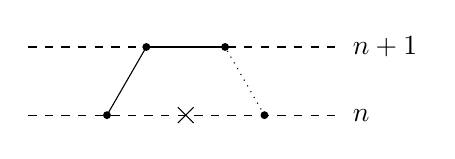
\begin{tikzpicture}
        \draw [dashed] (-1.0, 0.0) -- (3.0, 0.0);
        \fill (3.0, 0.0) node [right] {$n$};
        \draw [dashed] (-1.0, 0.866) -- (3.0, 0.866);
        \fill (3.0, 0.866) node [right] {$n+1$};
        \fill (0,0) circle [radius = 0.05];
        \begin{scope}[shift = (0 : 1.0)]
          \draw (-0.1,-0.1) -- (0.1,0.1);
          \draw (0.1,-0.1) -- (-0.1,0.1);
          \foreach \theta in {0, 60, 120}{
            \fill (0,0) [transform canvas = {shift = (\theta : 1.0)}] circle [radius = 0.05];
          }
        \end{scope}
        \begin{scope}[shift = (60 : 1.0)]
          \draw (0 : 0.0) -- (240 : 1.0);
          \draw (0 : 0.0) -- (0 : 1.0);
        \end{scope}
        \begin{scope}[shift = (0 : 2.0)]
          \draw [dotted] (0 : 0.0) -- (120 : 1.0);
        \end{scope}
      \end{tikzpicture}
    \end{tabular}
    \caption{}
  \end{center}
\end{figure}

If there are no beads which can make a hydrogen bond after the first bead is fixed on a side of an equilateral hexagon with a radius of $n+1$, there will be two possibilities which a second bead is fixed, such as in Fig.2. That is, it should make two hydrogen bonds after Fig.1. because the two possibilities in Fig.2. are nondeterministic.

\begin{figure}
  \begin{center}
    \begin{tabular}{cc}
      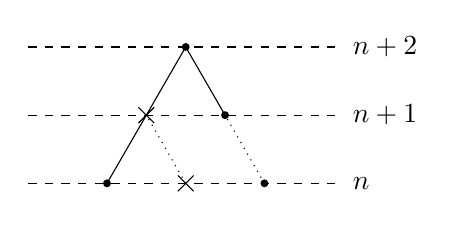
\begin{tikzpicture}
        \draw [dashed] (-1.0, 0.0) -- (3.0, 0.0);
        \fill (3.0, 0.0) node [right] {$n$};
        \draw [dashed] (-1.0, 0.866) -- (3.0, 0.866);
        \fill (3.0, 0.866) node [right] {$n+1$};
        \draw [dashed] (-1.0, 1.732) -- (3.0, 1.732);
        \fill (3.0, 1.732) node [right] {$n+2$};
        \fill (0,0) circle [radius = 0.05];
        \fill (60 : 2.0) circle [radius = 0.05];
        \begin{scope}[shift = (0 : 1.0)]
          \draw (-0.1,-0.1) -- (0.1,0.1);
          \draw (0.1,-0.1) -- (-0.1,0.1);
          \foreach \theta in {0, 60}{
            \fill (0,0) [transform canvas = {shift = (\theta : 1.0)}] circle [radius = 0.05];
          }
          \draw [dotted] (0 : 0.0) -- (120 : 1.0);
        \end{scope}
        \begin{scope}[shift = (60 : 1.0)]
          \draw (-0.1,-0.1) -- (0.1,0.1);
          \draw (0.1,-0.1) -- (-0.1,0.1);
          \draw (0 : 0.0) -- (240 : 1.0);
        \end{scope}
        \begin{scope}[shift = (0 : 2.0)]
          \draw [dotted] (0 : 0.0) -- (120 : 1.0);
        \end{scope}
        \begin{scope}[shift = (60 : 2.0)]
          \draw (0 : 0.0) -- (240 : 1.0);
          \draw (0 : 0.0) -- (300 : 1.0);
        \end{scope}
      \end{tikzpicture}

      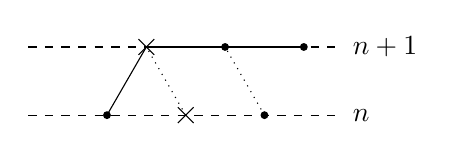
\begin{tikzpicture}
        \draw [dashed] (-1.0, 0.0) -- (3.0, 0.0);
        \fill (3.0, 0.0) node [right] {$n$};
        \draw [dashed] (-1.0, 0.866) -- (3.0, 0.866);
        \fill (3.0, 0.866) node [right] {$n+1$};
        \fill (0,0) circle [radius = 0.05];
        \begin{scope}[shift = (0 : 1.0)]
          \draw (-0.1,-0.1) -- (0.1,0.1);
          \draw (0.1,-0.1) -- (-0.1,0.1);
          \foreach \theta in {0, 60}{
            \fill (0,0) [transform canvas = {shift = (\theta : 1.0)}] circle [radius = 0.05];
          }
          \draw [dotted] (0 : 0.0) -- (120 : 1.0);
        \end{scope}
        \begin{scope}[shift = (60 : 1.0)]
          \draw (-0.1,-0.1) -- (0.1,0.1);
          \draw (0.1,-0.1) -- (-0.1,0.1);
          \draw (0 : 0.0) -- (240 : 1.0);
          \draw (0 : 0.0) -- (0 : 2.0);
          \fill (0 : 2.0) circle [radius = 0.05];
        \end{scope}
        \begin{scope}[shift = (0 : 2.0)]
          \draw [dotted] (0 : 0.0) -- (120 : 1.0);
        \end{scope}
      \end{tikzpicture}
    \end{tabular}
    \caption{}
  \end{center}
\end{figure}

Therefore, it should be a right or left figure in Fig.3. However, if it made two hydrogen bonds such as in Fig.3. once, it will make two hydrogen bonds forever to be deterministic. This becomes nondeterministic finally, such as in Fig.4., when it reaches a corner of an equilateral hexagon. 

\begin{figure}
  \begin{center}
  \begin{tabular}{cc}
    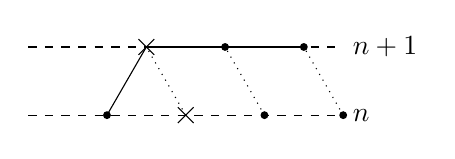
\begin{tikzpicture}
      \draw [dashed] (-1.0, 0.0) -- (3.0, 0.0);
      \fill (3.0, 0.0) node [right] {$n$};
      \draw [dashed] (-1.0, 0.866) -- (3.0, 0.866);
      \fill (3.0, 0.866) node [right] {$n+1$};
      \fill (0,0) circle [radius = 0.05];
      \begin{scope}[shift = (0 : 1.0)]
        \draw (-0.1,-0.1) -- (0.1,0.1);
        \draw (0.1,-0.1) -- (-0.1,0.1);
        \foreach \theta in {0, 60}{
          \fill (0,0) [transform canvas = {shift = (\theta : 1.0)}] circle [radius = 0.05];
        }
        \draw [dotted] (0 : 0.0) -- (120 : 1.0);
      \end{scope}
      \begin{scope}[shift = (60 : 1.0)]
        \draw (-0.1,-0.1) -- (0.1,0.1);
        \draw (0.1,-0.1) -- (-0.1,0.1);
        \draw (0 : 0.0) -- (240 : 1.0);
        \draw (0 : 0.0) -- (0 : 2.0);
        \fill (0 : 2.0) circle [radius = 0.05];
      \end{scope}
      \begin{scope}[shift = (0 : 2.0)]
        \draw [dotted] (0 : 0.0) -- (120 : 1.0);
      \end{scope}
      \begin{scope}[shift = (0 : 3.0)]
      \fill (0,0) circle [radius = 0.05];
        \draw [dotted] (0 : 0.0) -- (120 : 1.0);
      \end{scope}
    \end{tikzpicture}

    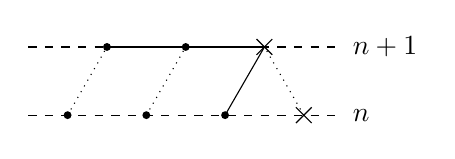
\begin{tikzpicture}
      \draw [dashed] (-2.5, 0.0) -- (1.5, 0.0);
      \fill (1.5, 0.0) node [right] {$n$};
      \draw [dashed] (-2.5, 0.866) -- (1.5, 0.866);
      \fill (1.5, 0.866) node [right] {$n+1$};
      \fill (0,0) circle [radius = 0.05];
      \fill (-1.0,0) circle [radius = 0.05];
      \begin{scope}[shift = (0 : 1.0)]
        \draw (-0.1,-0.1) -- (0.1,0.1);
        \draw (0.1,-0.1) -- (-0.1,0.1);
        \draw [dotted] (0 : 0.0) -- (120 : 1.0);
      \end{scope}
      \begin{scope}[shift = (60 : 1.0)]
        \draw (-0.1,-0.1) -- (0.1,0.1);
        \draw (0.1,-0.1) -- (-0.1,0.1);
        \draw (0 : 0.0) -- (240 : 1.0);
        \draw (0 : 0.0) -- (0 : -2.0);
        \fill (0 : -1.0) circle [radius = 0.05];
        \fill (0 : -2.0) circle [radius = 0.05];
      \end{scope}
      \begin{scope}[shift = (0 : -1.0)]
        \draw [dotted] (0 : 0.0) -- (60 : 1.0);
      \end{scope}
      \begin{scope}[shift = (0 : -2.0)]
      \fill (0,0) circle [radius = 0.05];
        \draw [dotted] (0 : 0.0) -- (60 : 1.0);
      \end{scope}
    \end{tikzpicture}
    \end{tabular}
    \caption{}
  \end{center}
\end{figure}

\begin{figure}
  \begin{center}
  \begin{tabular}{cc}
    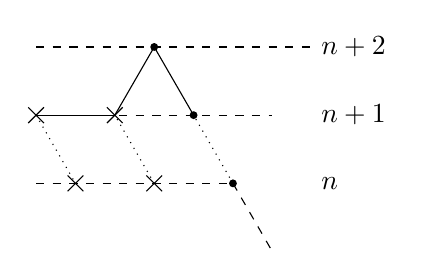
\begin{tikzpicture}
      \draw [dashed] (-0.5, 0.0) -- (2.0, 0.0);
      \fill (3.0, 0.0) node [right] {$n$};
      \draw [dashed] (-0.5, 0.866) -- (2.5, 0.866);
      \fill (3.0, 0.866) node [right] {$n+1$};
      \draw [dashed] (-0.5, 1.732) -- (3.0, 1.732);
      \fill (3.0, 1.732) node [right] {$n+2$};
      \fill (60 : 2.0) circle [radius = 0.05];
      \draw (-0.1,-0.1) -- (0.1,0.1);
      \draw (0.1,-0.1) -- (-0.1,0.1);
      \begin{scope}[shift = (120 : 1.0)]
        \draw (-0.1,-0.1) -- (0.1,0.1);
        \draw (0.1,-0.1) -- (-0.1,0.1);
      \end{scope}
      \begin{scope}[shift = (120 : 1.0)]
        \draw [dotted] (0 : 0.0) -- (300 : 1.0);
        \draw (0.0, 0.0) -- (1.0, 0.0);
      \end{scope}
      \begin{scope}[shift = (0 : 2.0)]
        \draw [dashed] (0 : 0.0) -- (300 : 1.0);
      \end{scope}
      \begin{scope}[shift = (0 : 1.0)]
        \draw (-0.1,-0.1) -- (0.1,0.1);
        \draw (0.1,-0.1) -- (-0.1,0.1);
        \foreach \theta in {0, 60}{
          \fill (0,0) [transform canvas = {shift = (\theta : 1.0)}] circle [radius = 0.05];
        }
        \draw [dotted] (0 : 0.0) -- (120 : 1.0);
      \end{scope}
      \begin{scope}[shift = (60 : 1.0)]
        \draw (-0.1,-0.1) -- (0.1,0.1);
        \draw (0.1,-0.1) -- (-0.1,0.1);
      \end{scope}
      \begin{scope}[shift = (0 : 2.0)]
        \draw [dotted] (0 : 0.0) -- (120 : 1.0);
      \end{scope}
      \begin{scope}[shift = (60 : 2.0)]
        \draw (0 : 0.0) -- (240 : 1.0);
        \draw (0 : 0.0) -- (300 : 1.0);
      \end{scope}
    \end{tikzpicture}

    \begin{tikzpicture}
      \draw [dashed] (-0.5, 0.0) -- (2.0, 0.0);
      \fill (3.0, 0.0) node [right] {$n$};
      \draw [dashed] (-0.5, 0.866) -- (2.5, 0.866);
      \fill (3.0, 0.866) node [right] {$n+1$};
      \draw (-0.1,-0.1) -- (0.1,0.1);
      \draw (0.1,-0.1) -- (-0.1,0.1);
      \begin{scope}[shift = (120 : 1.0)]
        \draw (-0.1,-0.1) -- (0.1,0.1);
        \draw (0.1,-0.1) -- (-0.1,0.1);
      \end{scope}
      \begin{scope}[shift = (120 : 1.0)]
        \draw [dotted] (0 : 0.0) -- (300 : 1.0);
        \draw (0.0, 0.0) -- (3.0, 0.0);
      \end{scope}
      \begin{scope}[shift = (0 : 2.0)]
        \draw [dashed] (0 : 0.0) -- (300 : 1.0);
        \fill (60 : 1.0) circle [radius = 0.05];
      \end{scope}
      \begin{scope}[shift = (0 : 1.0)]
        \draw (-0.1,-0.1) -- (0.1,0.1);
        \draw (0.1,-0.1) -- (-0.1,0.1);
        \foreach \theta in {0, 60}{
          \fill (0,0) [transform canvas = {shift = (\theta : 1.0)}] circle [radius = 0.05];
        }
        \draw [dotted] (0 : 0.0) -- (120 : 1.0);
      \end{scope}
      \begin{scope}[shift = (60 : 1.0)]
        \draw (-0.1,-0.1) -- (0.1,0.1);
        \draw (0.1,-0.1) -- (-0.1,0.1);
      \end{scope}
      \begin{scope}[shift = (0 : 2.0)]
        \draw [dotted] (0 : 0.0) -- (120 : 1.0);
      \end{scope}
    \end{tikzpicture}
    \end{tabular}
    \caption{}
  \end{center}
\end{figure}



\subsection{In the case of $\delta = 3$}

We discuss when the length of seed is $n$. If the length of seed is $n$, the seed will be in an equilateral hexagon with a radius of $n$ when it is given. We will begin our disscussion by considering the moment when a first bead is fixed on a side of an equilateral hexagon with a radius of $n+1$. Let us assume that a fixed bead on a side of an equilateral hexagon with a radius of $n$ is able to make a hydrogen bond. If it is able to make only two hydrogen bonds, it will be nondeterministic because there are two possibilities that it makes two structures in Fig.5. Therefore, it needs to make three hydrogen bonds to determine the only structure.\\

\begin{figure}
  \begin{center}
  \begin{tabular}{cc}
    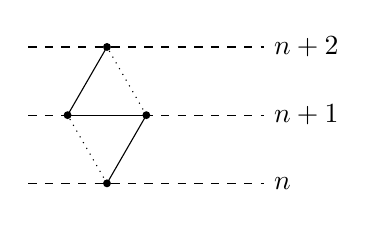
\begin{tikzpicture}
      \draw [dashed] (-1.0, 0.0) -- (2.0, 0.0);
      \fill (2.0, 0.0) node [right] {$n$};
      \draw [dashed] (-1.0, 0.866) -- (2.0, 0.866);
      \fill (2.0, 0.866) node [right] {$n+1$};
      \draw [dashed] (-1.0, 1.732) -- (2.0, 1.732);
      \fill (2.0, 1.732) node [right] {$n+2$};
      \fill (0,0) circle [radius = 0.05];
      \begin{scope}[shift = (0 : 0.0)]
        \foreach \theta in {60, 120}{
          \fill (0,0) [transform canvas = {shift = (\theta : 1.0)}] circle [radius = 0.05];
        }
        \draw (0 : 0.0) -- (60 : 1.0);
        \draw (60 : 1.0) -- (120 : 1.0);
        \draw [dotted] (0 : 0.0) -- (120 : 1.0);
      \end{scope}
      \begin{scope}[shift = (60 : 1.0)]
        \draw [dotted] (0 : 0.0) -- (120 : 1.0);
      \end{scope}
      \begin{scope}[shift = (120 : 1.0)]
        \foreach \theta in {60}{
        \fill (0,0) [transform canvas = {shift = (\theta : 1.0)}] circle [radius = 0.05];
        }
        \draw (0 : 0.0) -- (60 : 1.0);
      \end{scope}
    \end{tikzpicture}

    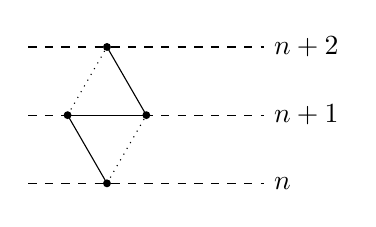
\begin{tikzpicture}
      \draw [dashed] (-1.0, 0.0) -- (2.0, 0.0);
      \fill (2.0, 0.0) node [right] {$n$};
      \draw [dashed] (-1.0, 0.866) -- (2.0, 0.866);
      \fill (2.0, 0.866) node [right] {$n+1$};
      \draw [dashed] (-1.0, 1.732) -- (2.0, 1.732);
      \fill (2.0, 1.732) node [right] {$n+2$};
      \fill (0,0) circle [radius = 0.05];
      \begin{scope}[shift = (0 : 0.0)]
        \foreach \theta in {60, 120}{
          \fill (0,0) [transform canvas = {shift = (\theta : 1.0)}] circle [radius = 0.05];
        }
        \draw [dotted] (0 : 0.0) -- (60 : 1.0);
        \draw (60 : 1.0) -- (120 : 1.0);
        \draw (0 : 0.0) -- (120 : 1.0);
      \end{scope}
      \begin{scope}[shift = (60 : 1.0)]
        \draw (0 : 0.0) -- (120 : 1.0);
      \end{scope}
      \begin{scope}[shift = (120 : 1.0)]
        \foreach \theta in {60}{
        \fill (0,0) [transform canvas = {shift = (\theta : 1.0)}] circle [radius = 0.05];
        }
        \draw [dotted](0 : 0.0) -- (60 : 1.0);
      \end{scope}
    \end{tikzpicture}
    \end{tabular}
    \caption{}
  \end{center}
\end{figure}

There are the two cases in which a first bead is fixed on a side of an equilateral hexagon with a radius of $n+1$ and it makes three hydrogen bonds in Fig.6. If it makes three hydrogen bonds once such as Fig6., it will make three hyrogen bonds forever to be deterministic. This becomes nondeterministic finally, such as in Fig.7., when it reaches a corner of an equilateral hexagon. Thus, the fixed bead on a side of an equilateral hexagon with a radius of $n$ has to make a hydrogen bond with a bead in an equilateral hexagon.

\begin{figure}
  \begin{center}
  \begin{tabular}{cc}
    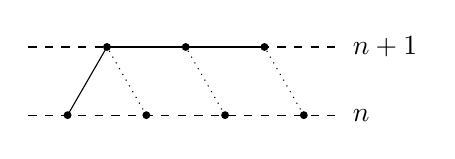
\begin{tikzpicture}
      \draw [dashed] (-0.5, 0.0) -- (3.5, 0.0);
      \fill (3.5, 0.0) node [right] {$n$};
      \draw [dashed] (-0.5, 0.866) -- (3.5, 0.866);
      \fill (3.5, 0.866) node [right] {$n+1$};
      \fill (0,0) circle [radius = 0.05];
      \begin{scope}[shift = (0 : 0.0)]
        \foreach \theta in {0, 60}{
          \fill (0,0) [transform canvas = {shift = (\theta : 1.0)}] circle [radius = 0.05];
        }
        \draw (0 : 0.0) -- (60 : 1.0);
      \end{scope}
      \begin{scope}[shift = (0 : 2.0)]
        \fill (0,0) circle [radius = 0.05];
        \foreach \theta in {0, 60, 120}{
          \fill (0,0) [transform canvas = {shift = (\theta : 1.0)}] circle [radius = 0.05];
        }
        \draw [dotted] (0 : 0.0) -- (120 : 1.0);
      \end{scope}
      \begin{scope}[shift = (60 : 1.0)]
          \draw (0 : 0.0) -- (0 : 2.0);
      \end{scope}
      \begin{scope}[shift = (0 : 1.0)]
          \draw [dotted] (0 : 0.0) -- (120 : 1.0);
      \end{scope}
      \begin{scope}[shift = (0 : 3.0)]
          \draw [dotted] (0 : 0.0) -- (120 : 1.0);
      \end{scope}
    \end{tikzpicture}

    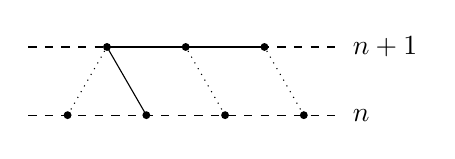
\begin{tikzpicture}
      \draw [dashed] (-1.5, 0.0) -- (2.5, 0.0);
      \fill (2.5, 0.0) node [right] {$n$};
      \draw [dashed] (-1.5, 0.866) -- (2.5, 0.866);
      \fill (2.5, 0.866) node [right] {$n+1$};
      \fill (0,0) circle [radius = 0.05];
      \begin{scope}[shift = (0 : 0.0)]
        \foreach \theta in {0, 60, 120, 180}{
          \fill (0,0) [transform canvas = {shift = (\theta : 1.0)}] circle [radius = 0.05];
        }
        \draw (0 : 0.0) -- (120 : 1.0);
      \end{scope}
      \begin{scope}[shift = (0 : 2.0)]
        \fill (0,0) circle [radius = 0.05];
        \foreach \theta in {120}{
          \fill (0,0) [transform canvas = {shift = (\theta : 1.0)}] circle [radius = 0.05];
        }
        \draw [dotted] (0 : 0.0) -- (120 : 1.0);
      \end{scope}
      \begin{scope}[shift = (120 : 1.0)]
          \draw (0 : 0.0) -- (0 : 2.0);
      \end{scope}
      \begin{scope}[shift = (0 : 1.0)]
          \draw [dotted] (0 : 0.0) -- (120 : 1.0);
      \end{scope}
      \begin{scope}[shift = (180 : 1.0)]
          \draw [dotted] (0 : 0.0) -- (60 : 1.0);
      \end{scope}
    \end{tikzpicture}
    \end{tabular}
    \caption{}
  \end{center}
\end{figure}

\begin{figure}
  \begin{center}
  \begin{tabular}{cc}
    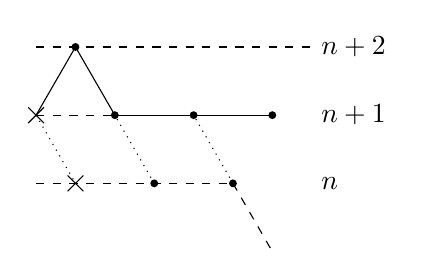
\begin{tikzpicture}
      \draw [dashed] (-0.5, 0.0) -- (2.0, 0.0);
      \fill (3.0, 0.0) node [right] {$n$};
      \draw [dashed] (-0.5, 0.866) -- (2.5, 0.866);
      \fill (3.0, 0.866) node [right] {$n+1$};
      \draw [dashed] (-0.5, 1.732) -- (3.0, 1.732);
      \fill (3.0, 1.732) node [right] {$n+2$};
      \fill (60 : 1.0) circle [radius = 0.05];
      \draw (-0.1,-0.1) -- (0.1,0.1);
      \draw (0.1,-0.1) -- (-0.1,0.1);
      \begin{scope}[shift = (120 : 1.0)]
        \draw (-0.1,-0.1) -- (0.1,0.1);
        \draw (0.1,-0.1) -- (-0.1,0.1);
      \end{scope}
      \begin{scope}[shift = (120 : 1.0)]
        \draw [dotted] (0 : 0.0) -- (300 : 1.0);
      \end{scope}
      \begin{scope}[shift = (60 : 1.0)]
        \draw (0.0, 0.0) -- (2.0, 0.0);
        \fill (2.0, 0.0) circle [radius = 0.05];
      \end{scope}
      \begin{scope}[shift = (0 : 2.0)]
        \draw [dashed] (0 : 0.0) -- (300 : 1.0);
      \end{scope}
      \begin{scope}[shift = (0 : 1.0)]
      \fill (0.0, 0.0) circle [radius = 0.05];
        \foreach \theta in {0, 60}{
          \fill (0,0) [transform canvas = {shift = (\theta : 1.0)}] circle [radius = 0.05];
        }
        \draw [dotted] (0 : 0.0) -- (120 : 1.0);
      \end{scope}
      \begin{scope}[shift = (0 : 2.0)]
        \draw [dotted] (0 : 0.0) -- (120 : 1.0);
      \end{scope}
      \begin{scope}[shift = (60 : 1.0)]
        \begin{scope}[shift = (120 : 1.0)]
          \fill (0.0, 0.0) circle [radius = 0.05];
          \draw (0 : 0.0) -- (240 : 1.0);
          \draw (0 : 0.0) -- (300 : 1.0);
        \end{scope}
      \end{scope}
    \end{tikzpicture}

    \begin{tikzpicture}
      \draw [dashed] (-0.5, 0.0) -- (2.0, 0.0);
      \fill (3.0, 0.0) node [right] {$n$};
      \draw [dashed] (-0.5, 0.866) -- (2.5, 0.866);
      \fill (3.0, 0.866) node [right] {$n+1$};
      \draw (-0.1,-0.1) -- (0.1,0.1);
      \draw (0.1,-0.1) -- (-0.1,0.1);
      \fill (60 : 1.0) circle [radius = 0.05];
      \begin{scope}[shift = (120 : 1.0)]
        \draw (-0.1,-0.1) -- (0.1,0.1);
        \draw (0.1,-0.1) -- (-0.1,0.1);
      \end{scope}
      \begin{scope}[shift = (120 : 1.0)]
        \draw [dotted] (0 : 0.0) -- (300 : 1.0);
        \draw (0.0, 0.0) -- (3.0, 0.0);
      \end{scope}
      \begin{scope}[shift = (0 : 2.0)]
        \draw [dashed] (0 : 0.0) -- (300 : 1.0);
        \fill (60 : 1.0) circle [radius = 0.05];
      \end{scope}
      \begin{scope}[shift = (0 : 1.0)]
        \fill (0.0, 0.0) circle [radius = 0.05];
        \foreach \theta in {0, 60}{
          \fill (0,0) [transform canvas = {shift = (\theta : 1.0)}] circle [radius = 0.05];
        }
        \draw [dotted] (0 : 0.0) -- (120 : 1.0);
      \end{scope}
      \begin{scope}[shift = (0 : 2.0)]
        \draw [dotted] (0 : 0.0) -- (120 : 1.0);
      \end{scope}
    \end{tikzpicture}
    \end{tabular}
    \caption{}
  \end{center}
\end{figure}

Then, we will discuss the moment after the first the is fixed on a side of an equilateral hexagon with a radius of $n+1$. Let us assume that the bead is able to make a hydrogen bond. If it is able to make only two hydrogen bonds, it will be nondeterministic because there are possibilities that it makes two structures in Fig.8. Hence, it needs to make three hydrogen bonds to determine the only structure. It needs to be a right or left figure in Fig.9. to make three hydrogen bonds.\\

\begin{figure}
  \begin{center}
  \begin{tabular}{cc}
    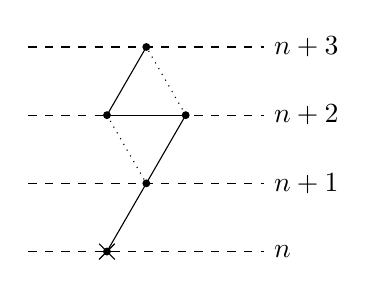
\begin{tikzpicture}
        \begin{scope}[shift=(0 : 0.0)]
          \draw (-0.1,-0.1) -- (0.1,0.1);
          \draw (0.1,-0.1) -- (-0.1,0.1);
          \draw (0 : 0.0) -- (60 : 1.0);
        \end{scope}
      \draw [dashed] (-1.0, 0.0) -- (2.0, 0.0);
      \fill (2.0, 0.0) node [right] {$n$};
      \draw [dashed] (-1.0, 0.866) -- (2.0, 0.866);
      \fill (2.0, 0.866) node [right] {$n+1$};
      \draw [dashed] (-1.0, 1.732) -- (2.0, 1.732);
      \fill (2.0, 1.732) node [right] {$n+2$};
      \draw [dashed] (-1.0, 2.598) -- (2.0, 2.598);
      \fill (2.0, 2.598) node [right] {$n+3$};
      \fill (0,0) circle [radius = 0.05];
      \begin{scope}[shift = (60 : 2.0)]
        \fill(0.0, 0.0) circle [radius = 0.05];
        \foreach \theta in {120, 180, 240}{
          \fill (0.0, 0.0) [transform canvas = {shift = (\theta : 1.0)}] circle [radius = 0.05];
        }
        \draw [dotted] (0 : 0.0) -- (120 : 1.0);
        \draw (0 : 0.0) -- (180 : 1.0);
        \draw (0 : 0.0) -- (240 : 1.0);
      \end{scope}
      \begin{scope}[shift = (60 : 1.0)]
        \begin{scope}[shift = (120 : 1.0)]
          \draw (0.0, 0.0) -- (60 : 1.0);
          \draw [dotted] (0.0, 0.0) -- (300 : 1.0);
        \end{scope}
      \end{scope}
    \end{tikzpicture}

    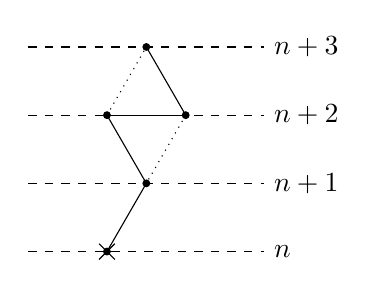
\begin{tikzpicture}
        \begin{scope}[shift=(0 : 0.0)]
          \draw (-0.1,-0.1) -- (0.1,0.1);
          \draw (0.1,-0.1) -- (-0.1,0.1);
          \draw (0 : 0.0) -- (60 : 1.0);
        \end{scope}
      \draw [dashed] (-1.0, 0.0) -- (2.0, 0.0);
      \fill (2.0, 0.0) node [right] {$n$};
      \draw [dashed] (-1.0, 0.866) -- (2.0, 0.866);
      \fill (2.0, 0.866) node [right] {$n+1$};
      \draw [dashed] (-1.0, 1.732) -- (2.0, 1.732);
      \fill (2.0, 1.732) node [right] {$n+2$};
      \draw [dashed] (-1.0, 2.598) -- (2.0, 2.598);
      \fill (2.0, 2.598) node [right] {$n+3$};
      \fill (0,0) circle [radius = 0.05];
      \begin{scope}[shift = (60 : 2.0)]
        \fill(0.0, 0.0) circle [radius = 0.05];
        \foreach \theta in {120, 180, 240}{
          \fill (0.0, 0.0) [transform canvas = {shift = (\theta : 1.0)}] circle [radius = 0.05];
        }
        \draw (0 : 0.0) -- (120 : 1.0);
        \draw (0 : 0.0) -- (180 : 1.0);
        \draw [dotted] (0 : 0.0) -- (240 : 1.0);
      \end{scope}
      \begin{scope}[shift = (60 : 1.0)]
        \begin{scope}[shift = (120 : 1.0)]
          \draw [dotted] (0.0, 0.0) -- (60 : 1.0);
          \draw (0.0, 0.0) -- (300 : 1.0);
        \end{scope}
      \end{scope}
    \end{tikzpicture}
    \end{tabular}
    \caption{}
  \end{center}
\end{figure}

 If it makes three hydrogen bonds once such as Fig.9., it will make three hyrogen bonds forever to be deterministic. This becomes nondeterministic finally, such as in Fig.7., when it reaches a corner of an equilateral hexagon. Therefore, the first fixed bead on a side of an equilateral hexagon with a radius of $n+1$ has to make a hydrogen bond with a molecule on a side of an equilateral hexagon with a radius of $n$.

\begin{figure}
  \begin{center}
  \begin{tabular}{cc}
    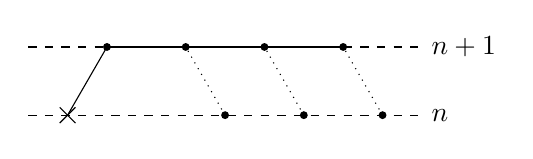
\begin{tikzpicture}
      \begin{scope}[shift=(0 : 0.0)]
        \draw (-0.1,-0.1) -- (0.1,0.1);
        \draw (0.1,-0.1) -- (-0.1,0.1);
        \draw (0 : 0.0) -- (60 : 1.0);
      \end{scope}
      \draw [dashed] (-0.5, 0.0) -- (4.5, 0.0);
      \fill (4.5, 0.0) node [right] {$n$};
      \draw [dashed] (-0.5, 0.866) -- (4.5, 0.866);
      \fill (4.5, 0.866) node [right] {$n+1$};
      \fill (2.0, 0.0) circle [radius = 0.05];
      \fill (3.0, 0.0) circle [radius = 0.05];
      \fill (4.0, 0.0) circle [radius = 0.05];
      \begin{scope}[shift = (60 : 1.0)]
        \fill (0.0, 0.0) circle [radius = 0.05];
        \fill (1.0, 0.0) circle [radius = 0.05];
        \fill (2.0, 0.0) circle [radius = 0.05];
        \fill (3.0, 0.0) circle [radius = 0.05];
        \draw (0.0, 0.0) -- (3.0, 0.0);
      \end{scope}
      \begin{scope}[shift = (0 : 2.0)]
        \draw [dotted] (0 : 0.0) -- (120 : 1.0);
      \end{scope}
      \begin{scope}[shift = (0 : 3.0)]
        \draw [dotted] (0 : 0.0) -- (120 : 1.0);
      \end{scope}
      \begin{scope}[shift = (0 : 4.0)]
        \draw [dotted] (0 : 0.0) -- (120 : 1.0);
      \end{scope}
    \end{tikzpicture}

    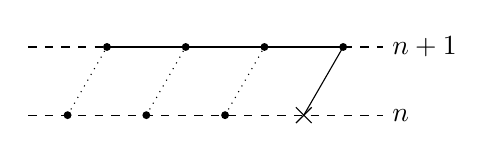
\begin{tikzpicture}
      \begin{scope}[shift=(0 : 0.0)]
        \draw (-0.1,-0.1) -- (0.1,0.1);
        \draw (0.1,-0.1) -- (-0.1,0.1);
        \draw (0 : 0.0) -- (60 : 1.0);
      \end{scope}
      \draw [dashed] (-3.5, 0.0) -- (1.0, 0.0);
      \fill (1.0, 0.0) node [right] {$n$};
      \draw [dashed] (-3.5, 0.866) -- (1.0, 0.866);
      \fill (1.0, 0.866) node [right] {$n+1$};
      \fill (-1.0, 0.0) circle [radius = 0.05];
      \fill (-2.0, 0.0) circle [radius = 0.05];
      \fill (-3.0, 0.0) circle [radius = 0.05];
      \begin{scope}[shift = (60 : 1.0)]
        \fill (0.0, 0.0) circle [radius = 0.05];
        \fill (-1.0, 0.0) circle [radius = 0.05];
        \fill (-2.0, 0.0) circle [radius = 0.05];
        \fill (-3.0, 0.0) circle [radius = 0.05];
        \draw (0.0, 0.0) -- (-3.0, 0.0);
      \end{scope}
      \begin{scope}[shift = (0 : -1.0)]
        \draw [dotted] (0 : 0.0) -- (60 : 1.0);
      \end{scope}
      \begin{scope}[shift = (0 : -2.0)]
        \draw [dotted] (0 : 0.0) -- (60 : 1.0);
      \end{scope}
      \begin{scope}[shift = (0 : -3.0)]
        \draw [dotted] (0 : 0.0) -- (60 : 1.0);
      \end{scope}
    \end{tikzpicture}
    \end{tabular}
    \caption{}
  \end{center}
\end{figure}

Accordingly, it is Fig.10. when a first bead is fixed on a side of an equilateral hexagon with a radius of $n+1$.

\begin{figure}
  \begin{center}
    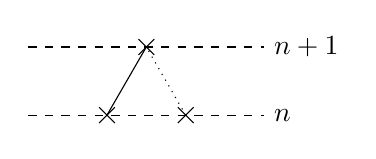
\begin{tikzpicture}
      \draw [dashed] (-1.0, 0.0) -- (2.0, 0.0);
      \fill (2.0, 0.0) node [right] {$n$};
      \draw [dashed] (-1.0, 0.866) -- (2.0, 0.866);
      \fill (2.0, 0.866) node [right] {$n+1$};
      \begin{scope}[shift=(0 : 0.0)]
        \draw (-0.1,-0.1) -- (0.1,0.1);
        \draw (0.1,-0.1) -- (-0.1,0.1);
        \draw (0 : 0.0) -- (60 : 1.0);
      \end{scope}
      \begin{scope}[shift=(60 : 1.0)]
        \draw (-0.1,-0.1) -- (0.1,0.1);
        \draw (0.1,-0.1) -- (-0.1,0.1);
      \end{scope}
      \begin{scope}[shift=(0 : 1.0)]
        \draw (-0.1,-0.1) -- (0.1,0.1);
        \draw (0.1,-0.1) -- (-0.1,0.1);
        \draw [dotted] (0 : 0.0) -- (120 : 1.0);
      \end{scope}
    \end{tikzpicture}
    \caption{}
  \end{center}
\end{figure}

It has to be a right or left figure in Fig.6. when the first bead fixed on a side of an equilateral hexagon with a radius of $n+1$ make a hydrogen bond with a bead on a side of an equilateral hexagon with a radius of $n$. Fig.6. becomes nondeterministic finally, such as in Fig.7., when it reaches a corner of an equilateral hexagon. It is clear that all beads on a side of an equilateral hexagon with a radius of $n+1$ has to make a hydrogen bond with a bead on a side of an equilateral hexagon with a radius of $n$.  It is impossible to fix molecules on a side of an equilateral hexagon with a radius of $n+2$ and determine the only structure when there are only beads which are able to make a hydrogen bond in an equilateral hexagon with a radius of $n$.


\end{document}